\documentclass[aps,prb,onecolumn,notitlepage,showpacs,floatfix,superscriptaddress]{revtex4-1}
\usepackage{dcolumn}
\usepackage{tabularx}
\usepackage{bm}
\usepackage{soul}
\usepackage{amsmath,xcolor}
\fboxrule=1pt
\usepackage{amssymb,graphicx}
\usepackage[colorlinks=true,citecolor=blue,urlcolor=blue,linkcolor=blue]{hyperref}
\usepackage{environ}

\usepackage{tikz}
\usetikzlibrary{matrix}
\usetikzlibrary{fit}

\NewEnviron{eqnsplit}{%
\begin{equation}
\begin{split}
  \BODY
\end{split}
\end{equation}
}
\newcommand{\mrm}[1]{\mathrm{#1}}
\newcommand{\AR}[1]{\textcolor{red}{#1}}
\newcommand{\ang}{\mathrm{\AA}}

\bibliographystyle{apsrev4-1}

%%%%%%%%%%%%%%%%%%%%%%%%%%%%%%%%%%%%%%%%%%%%%%%%
\begin{document}
\title{Skyrmions: Emergent Fields}

\author{Avinash Rustagi}
\email{arustag@purdue.edu}
%
%\date{\today}
%%%%%%%%%%%%%%%%%%%%%%%%%%%%%%%%%%%%%%%%%%%%%%%%

\maketitle
%
\begin{figure}[hbtp]
\centering
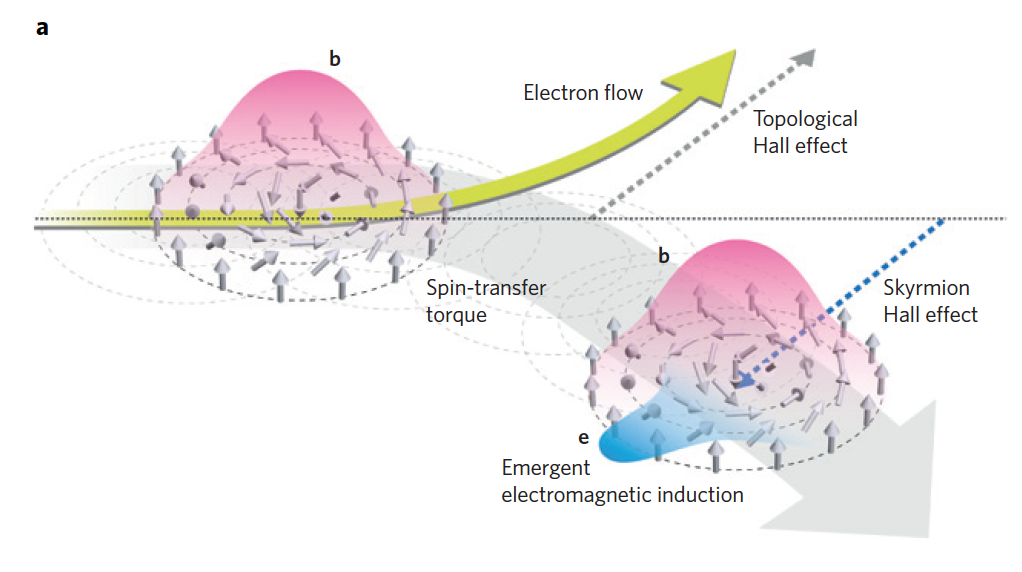
\includegraphics[width=0.6\textwidth]{Schematic.png}
\caption{Schematic for phenomenon arising from non-trivial topology of skyrmions. Ref: `Topological properties and dynamics of magnetic skyrmions'- Nagaosa and Tokura, Nature Nanotechnology 8, 899 (2013)}
\end{figure}

We understand the non-trivial topology of skyrmion magnetic textures. Here, we would like to consider the emergent EM field that a propagating conduction electron experiences when traversing through such a topological texture. To develop a simplistic understanding, we assume that there is a strong Hund's exchange coupling between the electron and local magnetization. As a consequence of this strong coupling, the spin part of the wavefunction of the conduction electron is oriented in parallel to the local magnetization, such that
\begin{equation}
\vert \chi (\vec{r}) \rangle = \left( \begin{array}{c}
\cos\dfrac{\Theta}{2} \\ 
e^{i\Phi} \sin\dfrac{\Theta}{2}
\end{array} \right)
\end{equation}
where $\Theta$ and $\Phi$ describe the orientation of the local magnetization. The motion of a electron in a lattice is described in terms of a hopping matrix element (in tight binding model). Such a hopping as a result of lattice translations along different directions $\alpha$ can be computed
\begin{equation}
t_\alpha (\vec{r}) = t \langle \chi(\vec{r}) \vert \chi(\vec{r}+c\hat{\eta}_\alpha) \rangle
\end{equation}
where $t$ is the bare hopping, $c$ is the lattice constant. A simple series expansion
\begin{equation}
\vert \chi(\vec{r}+c\hat{\eta}_\alpha) \rangle \approx \vert \chi(\vec{r}) \rangle + c \, \partial_\alpha \vert \chi(\vec{r}) \rangle
\end{equation}
Consequently,
\begin{equation}
\begin{split}
t_\alpha (\vec{r}) &= t [1 + c \, \langle \chi(\vec{r}) \vert \partial_\alpha \chi(\vec{r}) \rangle] \\
&= t e^{ic\, a_{\alpha} (\vec{r})}
\end{split}
\end{equation}
where $a_{\alpha} (\vec{r}) = -i\langle \chi(\vec{r}) \vert \partial_\alpha \chi(\vec{r}) \rangle$ is the effective vector potential experienced by the electron. Utilizing
\begin{equation}
\vert \partial_\alpha \chi (\vec{r}) \rangle = \left( \begin{array}{c}
-\dfrac{1}{2}\sin\dfrac{\Theta}{2} \partial_\alpha\Theta \\ 
i \partial_\alpha \Phi e^{i\Phi} \sin\dfrac{\Theta}{2} + \dfrac{1}{2}e^{i\Phi}\cos\dfrac{\Theta}{2} \partial_\alpha\Theta 
\end{array} \right)
\end{equation}
implies
\begin{equation}
a_{\alpha} (\vec{r}) = \dfrac{1}{2} \partial_\alpha \Phi [1-\cos\Theta]
\end{equation}
We can look at the out-of-plane magnetic field originating from the emergent vector potential
\begin{equation}
b_z = \partial_x a_y - \partial_y a_x = \dfrac{1}{2} \vec{m} \cdot (\partial_x \vec{m} \times \partial_y \vec{m})
\end{equation}
Consequently, the magnetic flux thought the x-y plane corresponding to the magnetic field is related to the topological skyrmion charge
\begin{equation}
\Phi_B = 2\pi \, Q_\mrm{sk}
\end{equation}
A consequence of this emergent magnetic field leads to a Hall effect referred to as `Topological Hall Effect'. On the other hand, electron charge current applies a spin transfer torque (STT) which due to the presence of Gyrovector causes the skyrmion to move transverse to the direction of electric current. This is referred to as the `Skyrmion Hall Effect'.\\

\noindent To determine the emergent electric field in addition to the magnetic field described above, we can alternatively look at the Schrodinger equation for the electron,
\begin{equation}
i \partial_t \psi(\vec{r},t) = \left[-\dfrac{\nabla^2}{2m} - J \vec{\sigma} \cdot \vec{m} \right] \psi(\vec{r},t)
\end{equation}
The problem gets easier to tackle if the spin quantization axis aligns with the local magnetization orientation. To do so, we can perform a unitary transformation corresponding to rotation by an angle $\Theta(\vec{r},t)$ about an axis that is normal to both the z-axis and the local magnetization orientation $\hat{n} = \hat{z} \times \vec{m}$,
\begin{equation}
U(\vec{r},t) = \exp\left( -i \dfrac{\Theta(\vec{r},t)}{2} \vec{\sigma} \cdot \hat{n}(\vec{r},t)\right)
\end{equation}
We can now rewrite the Schrodinger equation in terms of wavefunction $\phi(\vec{r},t)$ such that $\psi(\vec{r},t) = U(\vec{r},t) \phi(\vec{r},t)$,
\begin{widetext}
\begin{equation}
i \partial_t \phi(\vec{r},t) + [iU^\dagger \partial_t U] \phi(\vec{r},t) = \left[\dfrac{(-i\nabla - i U^\dagger \nabla U)^2}{2m} - J \sigma_z \right] \phi(\vec{r},t)
\end{equation}
\end{widetext}
This is similar to the Schrodinger equation of a charged particle in presence of both scalar and vector potential,
\begin{widetext}
\begin{equation}
i \partial_t \phi(\vec{r},t) - q_e V(\vec{r},t) \phi(\vec{r},t) = \left[\dfrac{(-i\nabla - q_e \vec{A}(\vec{r},t))^2}{2m} - J \sigma_z \right] \phi(\vec{r},t)
\end{equation}
\end{widetext}
Thus, the emergent potentials are defined as
\begin{equation}
V(\vec{r},t) = -\dfrac{i}{q_e} U^\dagger \partial_t U; \quad \vec{A}(\vec{r},t) = -\dfrac{i}{q_e} U^\dagger \nabla U  
\end{equation}
The emergent charge $q_e = \pm 1/2$ depending on the upper/lower band of the charge. One can now determine the emergent fields from the potentials,
\begin{equation}
\begin{split}
B_i &= \epsilon_{ijk} \partial_j A_k = \dfrac{\epsilon_{ijk}}{2} \vec{m} \cdot (\partial_j \vec{m} \times \partial_k \vec{m}) \\
E_i &= -\partial_i V - \partial_t A_i = \vec{m} \cdot (\partial_i \vec{m} \times \partial_t \vec{m}) \\
\end{split}
\end{equation}
\end{document}
